% Options for packages loaded elsewhere
% Options for packages loaded elsewhere
\PassOptionsToPackage{unicode}{hyperref}
\PassOptionsToPackage{hyphens}{url}
\PassOptionsToPackage{dvipsnames,svgnames,x11names}{xcolor}
%
\documentclass[
  letterpaper,
  DIV=11,
  numbers=noendperiod]{scrartcl}
\usepackage{xcolor}
\usepackage{amsmath,amssymb}
\setcounter{secnumdepth}{-\maxdimen} % remove section numbering
\usepackage{iftex}
\ifPDFTeX
  \usepackage[T1]{fontenc}
  \usepackage[utf8]{inputenc}
  \usepackage{textcomp} % provide euro and other symbols
\else % if luatex or xetex
  \usepackage{unicode-math} % this also loads fontspec
  \defaultfontfeatures{Scale=MatchLowercase}
  \defaultfontfeatures[\rmfamily]{Ligatures=TeX,Scale=1}
\fi
\usepackage{lmodern}
\ifPDFTeX\else
  % xetex/luatex font selection
\fi
% Use upquote if available, for straight quotes in verbatim environments
\IfFileExists{upquote.sty}{\usepackage{upquote}}{}
\IfFileExists{microtype.sty}{% use microtype if available
  \usepackage[]{microtype}
  \UseMicrotypeSet[protrusion]{basicmath} % disable protrusion for tt fonts
}{}
\makeatletter
\@ifundefined{KOMAClassName}{% if non-KOMA class
  \IfFileExists{parskip.sty}{%
    \usepackage{parskip}
  }{% else
    \setlength{\parindent}{0pt}
    \setlength{\parskip}{6pt plus 2pt minus 1pt}}
}{% if KOMA class
  \KOMAoptions{parskip=half}}
\makeatother
% Make \paragraph and \subparagraph free-standing
\makeatletter
\ifx\paragraph\undefined\else
  \let\oldparagraph\paragraph
  \renewcommand{\paragraph}{
    \@ifstar
      \xxxParagraphStar
      \xxxParagraphNoStar
  }
  \newcommand{\xxxParagraphStar}[1]{\oldparagraph*{#1}\mbox{}}
  \newcommand{\xxxParagraphNoStar}[1]{\oldparagraph{#1}\mbox{}}
\fi
\ifx\subparagraph\undefined\else
  \let\oldsubparagraph\subparagraph
  \renewcommand{\subparagraph}{
    \@ifstar
      \xxxSubParagraphStar
      \xxxSubParagraphNoStar
  }
  \newcommand{\xxxSubParagraphStar}[1]{\oldsubparagraph*{#1}\mbox{}}
  \newcommand{\xxxSubParagraphNoStar}[1]{\oldsubparagraph{#1}\mbox{}}
\fi
\makeatother

\usepackage{color}
\usepackage{fancyvrb}
\newcommand{\VerbBar}{|}
\newcommand{\VERB}{\Verb[commandchars=\\\{\}]}
\DefineVerbatimEnvironment{Highlighting}{Verbatim}{commandchars=\\\{\}}
% Add ',fontsize=\small' for more characters per line
\usepackage{framed}
\definecolor{shadecolor}{RGB}{241,243,245}
\newenvironment{Shaded}{\begin{snugshade}}{\end{snugshade}}
\newcommand{\AlertTok}[1]{\textcolor[rgb]{0.68,0.00,0.00}{#1}}
\newcommand{\AnnotationTok}[1]{\textcolor[rgb]{0.37,0.37,0.37}{#1}}
\newcommand{\AttributeTok}[1]{\textcolor[rgb]{0.40,0.45,0.13}{#1}}
\newcommand{\BaseNTok}[1]{\textcolor[rgb]{0.68,0.00,0.00}{#1}}
\newcommand{\BuiltInTok}[1]{\textcolor[rgb]{0.00,0.23,0.31}{#1}}
\newcommand{\CharTok}[1]{\textcolor[rgb]{0.13,0.47,0.30}{#1}}
\newcommand{\CommentTok}[1]{\textcolor[rgb]{0.37,0.37,0.37}{#1}}
\newcommand{\CommentVarTok}[1]{\textcolor[rgb]{0.37,0.37,0.37}{\textit{#1}}}
\newcommand{\ConstantTok}[1]{\textcolor[rgb]{0.56,0.35,0.01}{#1}}
\newcommand{\ControlFlowTok}[1]{\textcolor[rgb]{0.00,0.23,0.31}{\textbf{#1}}}
\newcommand{\DataTypeTok}[1]{\textcolor[rgb]{0.68,0.00,0.00}{#1}}
\newcommand{\DecValTok}[1]{\textcolor[rgb]{0.68,0.00,0.00}{#1}}
\newcommand{\DocumentationTok}[1]{\textcolor[rgb]{0.37,0.37,0.37}{\textit{#1}}}
\newcommand{\ErrorTok}[1]{\textcolor[rgb]{0.68,0.00,0.00}{#1}}
\newcommand{\ExtensionTok}[1]{\textcolor[rgb]{0.00,0.23,0.31}{#1}}
\newcommand{\FloatTok}[1]{\textcolor[rgb]{0.68,0.00,0.00}{#1}}
\newcommand{\FunctionTok}[1]{\textcolor[rgb]{0.28,0.35,0.67}{#1}}
\newcommand{\ImportTok}[1]{\textcolor[rgb]{0.00,0.46,0.62}{#1}}
\newcommand{\InformationTok}[1]{\textcolor[rgb]{0.37,0.37,0.37}{#1}}
\newcommand{\KeywordTok}[1]{\textcolor[rgb]{0.00,0.23,0.31}{\textbf{#1}}}
\newcommand{\NormalTok}[1]{\textcolor[rgb]{0.00,0.23,0.31}{#1}}
\newcommand{\OperatorTok}[1]{\textcolor[rgb]{0.37,0.37,0.37}{#1}}
\newcommand{\OtherTok}[1]{\textcolor[rgb]{0.00,0.23,0.31}{#1}}
\newcommand{\PreprocessorTok}[1]{\textcolor[rgb]{0.68,0.00,0.00}{#1}}
\newcommand{\RegionMarkerTok}[1]{\textcolor[rgb]{0.00,0.23,0.31}{#1}}
\newcommand{\SpecialCharTok}[1]{\textcolor[rgb]{0.37,0.37,0.37}{#1}}
\newcommand{\SpecialStringTok}[1]{\textcolor[rgb]{0.13,0.47,0.30}{#1}}
\newcommand{\StringTok}[1]{\textcolor[rgb]{0.13,0.47,0.30}{#1}}
\newcommand{\VariableTok}[1]{\textcolor[rgb]{0.07,0.07,0.07}{#1}}
\newcommand{\VerbatimStringTok}[1]{\textcolor[rgb]{0.13,0.47,0.30}{#1}}
\newcommand{\WarningTok}[1]{\textcolor[rgb]{0.37,0.37,0.37}{\textit{#1}}}

\usepackage{longtable,booktabs,array}
\newcounter{none} % for unnumbered tables
\usepackage{calc} % for calculating minipage widths
% Correct order of tables after \paragraph or \subparagraph
\usepackage{etoolbox}
\makeatletter
\patchcmd\longtable{\par}{\if@noskipsec\mbox{}\fi\par}{}{}
\makeatother
% Allow footnotes in longtable head/foot
\IfFileExists{footnotehyper.sty}{\usepackage{footnotehyper}}{\usepackage{footnote}}
\makesavenoteenv{longtable}
\usepackage{graphicx}
\makeatletter
\newsavebox\pandoc@box
\newcommand*\pandocbounded[1]{% scales image to fit in text height/width
  \sbox\pandoc@box{#1}%
  \Gscale@div\@tempa{\textheight}{\dimexpr\ht\pandoc@box+\dp\pandoc@box\relax}%
  \Gscale@div\@tempb{\linewidth}{\wd\pandoc@box}%
  \ifdim\@tempb\p@<\@tempa\p@\let\@tempa\@tempb\fi% select the smaller of both
  \ifdim\@tempa\p@<\p@\scalebox{\@tempa}{\usebox\pandoc@box}%
  \else\usebox{\pandoc@box}%
  \fi%
}
% Set default figure placement to htbp
\def\fps@figure{htbp}
\makeatother





\setlength{\emergencystretch}{3em} % prevent overfull lines

\providecommand{\tightlist}{%
  \setlength{\itemsep}{0pt}\setlength{\parskip}{0pt}}



 


\usepackage{booktabs}
\usepackage{caption}
\usepackage{longtable}
\usepackage{colortbl}
\usepackage{array}
\usepackage{anyfontsize}
\usepackage{multirow}
\KOMAoption{captions}{tableheading}
\makeatletter
\@ifpackageloaded{caption}{}{\usepackage{caption}}
\AtBeginDocument{%
\ifdefined\contentsname
  \renewcommand*\contentsname{Table of contents}
\else
  \newcommand\contentsname{Table of contents}
\fi
\ifdefined\listfigurename
  \renewcommand*\listfigurename{List of Figures}
\else
  \newcommand\listfigurename{List of Figures}
\fi
\ifdefined\listtablename
  \renewcommand*\listtablename{List of Tables}
\else
  \newcommand\listtablename{List of Tables}
\fi
\ifdefined\figurename
  \renewcommand*\figurename{Figure}
\else
  \newcommand\figurename{Figure}
\fi
\ifdefined\tablename
  \renewcommand*\tablename{Table}
\else
  \newcommand\tablename{Table}
\fi
}
\@ifpackageloaded{float}{}{\usepackage{float}}
\floatstyle{ruled}
\@ifundefined{c@chapter}{\newfloat{codelisting}{h}{lop}}{\newfloat{codelisting}{h}{lop}[chapter]}
\floatname{codelisting}{Listing}
\newcommand*\listoflistings{\listof{codelisting}{List of Listings}}
\makeatother
\makeatletter
\makeatother
\makeatletter
\@ifpackageloaded{caption}{}{\usepackage{caption}}
\@ifpackageloaded{subcaption}{}{\usepackage{subcaption}}
\makeatother
\usepackage{bookmark}
\IfFileExists{xurl.sty}{\usepackage{xurl}}{} % add URL line breaks if available
\urlstyle{same}
\hypersetup{
  pdftitle={Measles Study},
  pdfauthor={William Cuthbert, Sebastien Montgrain, Adrian Antonelli},
  colorlinks=true,
  linkcolor={blue},
  filecolor={Maroon},
  citecolor={Blue},
  urlcolor={Blue},
  pdfcreator={LaTeX via pandoc}}


\title{Measles Study}
\author{William Cuthbert, Sebastien Montgrain, Adrian Antonelli}
\date{}
\begin{document}
\maketitle

\renewcommand*\contentsname{Table of Contents}
{
\setcounter{tocdepth}{3}
\tableofcontents
}

\begin{Shaded}
\begin{Highlighting}[]
\FunctionTok{library}\NormalTok{(tidyverse)}
\FunctionTok{library}\NormalTok{(ggplot2)}
\FunctionTok{library}\NormalTok{(forcats)}
\FunctionTok{library}\NormalTok{(scales)}
\FunctionTok{library}\NormalTok{(ggridges)}
\FunctionTok{library}\NormalTok{(gt)}
\FunctionTok{library}\NormalTok{(purrr)}
\NormalTok{cases\_month }\OtherTok{\textless{}{-}}\NormalTok{ readr}\SpecialCharTok{::}\FunctionTok{read\_csv}\NormalTok{(}\StringTok{\textquotesingle{}https://raw.githubusercontent.com/rfordatascience/tidytuesday/main/data/2025/2025{-}06{-}24/cases\_month.csv\textquotesingle{}}\NormalTok{)}
\NormalTok{cases\_year }\OtherTok{\textless{}{-}}\NormalTok{ readr}\SpecialCharTok{::}\FunctionTok{read\_csv}\NormalTok{(}\StringTok{\textquotesingle{}https://raw.githubusercontent.com/rfordatascience/tidytuesday/main/data/2025/2025{-}06{-}24/cases\_year.csv\textquotesingle{}}\NormalTok{)}
\end{Highlighting}
\end{Shaded}

\subsection{Does time of year impact measles cases
globally?}\label{does-time-of-year-impact-measles-cases-globally}

\begin{Shaded}
\begin{Highlighting}[]
\NormalTok{case\_ranking\_by\_months }\OtherTok{\textless{}{-}}\NormalTok{ cases\_month }\SpecialCharTok{|\textgreater{}}
  \FunctionTok{group\_by}\NormalTok{(month, region) }\SpecialCharTok{|\textgreater{}}
  \FunctionTok{filter}\NormalTok{(measles\_total }\SpecialCharTok{\textgreater{}=} \DecValTok{0}\NormalTok{) }\SpecialCharTok{|\textgreater{}}
  \FunctionTok{summarise}\NormalTok{(}\AttributeTok{avg\_measles =} \FunctionTok{mean}\NormalTok{(measles\_total, }\AttributeTok{na.rm =} \ConstantTok{TRUE}\NormalTok{), }\AttributeTok{.groups =} \StringTok{"drop"}\NormalTok{) }\SpecialCharTok{|\textgreater{}}
  \FunctionTok{mutate}\NormalTok{(}\AttributeTok{month =} \FunctionTok{factor}\NormalTok{(month.abb[month], }\AttributeTok{levels =}\NormalTok{ month.abb),}
         \AttributeTok{region =} \FunctionTok{recode}\NormalTok{(region, }\StringTok{"AFR"} \OtherTok{=} \StringTok{"Africa"}\NormalTok{, }
                         \StringTok{"AMR"} \OtherTok{=} \StringTok{"Americas"}\NormalTok{, }
                         \StringTok{"EMR"} \OtherTok{=} \StringTok{"Eastern Mediterranean"}\NormalTok{, }
                         \StringTok{"EUR"} \OtherTok{=} \StringTok{"Europe"}\NormalTok{, }
                         \StringTok{"SEAR"} \OtherTok{=} \StringTok{"South{-}East Asia"}\NormalTok{, }
                         \StringTok{"WPR"} \OtherTok{=} \StringTok{"Western Pacific"}\NormalTok{)) }

\NormalTok{case\_ranking\_by\_months }\SpecialCharTok{|\textgreater{}}
  \FunctionTok{pivot\_wider}\NormalTok{(}\AttributeTok{names\_from =} \StringTok{"month"}\NormalTok{,}
              \AttributeTok{values\_from =} \StringTok{"avg\_measles"}\NormalTok{) }\SpecialCharTok{|\textgreater{}}
  \FunctionTok{gt}\NormalTok{() }\SpecialCharTok{|\textgreater{}}
  \FunctionTok{fmt\_number}\NormalTok{(}\AttributeTok{columns =} \FunctionTok{where}\NormalTok{(is.numeric), }\AttributeTok{decimals =} \DecValTok{2}\NormalTok{) }\SpecialCharTok{|\textgreater{}}
  \FunctionTok{cols\_label}\NormalTok{(}\AttributeTok{region =} \StringTok{"Region"}\NormalTok{) }\SpecialCharTok{|\textgreater{}}
  \FunctionTok{tab\_header}\NormalTok{(}\AttributeTok{title =} \StringTok{"Average Monthly Measles Cases by Region"}\NormalTok{) }\SpecialCharTok{|\textgreater{}}
  \FunctionTok{tab\_style}\NormalTok{(}\AttributeTok{style =} \FunctionTok{cell\_text}\NormalTok{(}\AttributeTok{weight =} \StringTok{"bold"}\NormalTok{),}
            \AttributeTok{locations =} \FunctionTok{cells\_title}\NormalTok{(}\AttributeTok{groups =} \StringTok{"title"}\NormalTok{))}
\end{Highlighting}
\end{Shaded}

\begin{table}
\caption*{
{\fontsize{20}{25}\selectfont  Average Monthly Measles Cases by Region\fontsize{12}{15}\selectfont }
} 
\fontsize{12.0pt}{14.0pt}\selectfont
\begin{tabular*}{\linewidth}{@{\extracolsep{\fill}}lrrrrrrrrrrrr}
\toprule
Region & Jan & Feb & Mar & Apr & May & Jun & Jul & Aug & Sep & Oct & Nov & Dec \\ 
\midrule\addlinespace[2.5pt]
Africa & 248.31 & 313.85 & 318.62 & 184.59 & 114.49 & 75.72 & 64.39 & 64.87 & 58.67 & 64.80 & 71.53 & 62.07 \\ 
Americas & 9.85 & 14.27 & 22.53 & 19.38 & 13.85 & 8.92 & 16.85 & 25.35 & 29.86 & 26.83 & 37.91 & 13.82 \\ 
Eastern Mediterranean & 197.64 & 220.18 & 254.11 & 220.38 & 226.71 & 170.83 & 135.83 & 105.42 & 103.08 & 105.32 & 110.66 & 112.92 \\ 
Europe & 132.05 & 131.76 & 131.87 & 122.39 & 112.67 & 80.01 & 53.27 & 32.80 & 30.66 & 45.29 & 58.07 & 88.87 \\ 
South-East Asia & 535.49 & 544.13 & 626.14 & 536.82 & 376.78 & 256.74 & 228.25 & 242.93 & 240.21 & 273.91 & 345.52 & 380.66 \\ 
Western Pacific & 231.52 & 278.21 & 333.09 & 308.29 & 307.14 & 206.20 & 135.85 & 108.47 & 76.58 & 71.48 & 80.07 & 57.88 \\ 
\bottomrule
\end{tabular*}
\end{table}

Table 1

\begin{Shaded}
\begin{Highlighting}[]
\FunctionTok{ggplot}\NormalTok{(case\_ranking\_by\_months, }\FunctionTok{aes}\NormalTok{(}\AttributeTok{x =}\NormalTok{ month, }\AttributeTok{y =}\NormalTok{ avg\_measles, }\AttributeTok{group =}\NormalTok{ region, }\AttributeTok{color =}\NormalTok{ region)) }\SpecialCharTok{+}
  \FunctionTok{geom\_line}\NormalTok{() }\SpecialCharTok{+}
  \FunctionTok{geom\_smooth}\NormalTok{(}\AttributeTok{method =} \StringTok{"lm"}\NormalTok{, }\AttributeTok{se =} \ConstantTok{FALSE}\NormalTok{,}
              \AttributeTok{linewidth =} \FloatTok{0.5}\NormalTok{,}
              \AttributeTok{linetype =} \StringTok{"dashed"}\NormalTok{,}
              \AttributeTok{col =} \StringTok{"black"}\NormalTok{) }\SpecialCharTok{+}
  \FunctionTok{facet\_wrap}\NormalTok{(}\SpecialCharTok{\textasciitilde{}}\NormalTok{region, }\AttributeTok{scales =} \StringTok{"free\_y"}\NormalTok{) }\SpecialCharTok{+}
  \FunctionTok{labs}\NormalTok{(}\AttributeTok{x =} \StringTok{"Month"}\NormalTok{, }\AttributeTok{title =} \StringTok{"Measles Cases by Month Across the World"}\NormalTok{, }\AttributeTok{y =} \StringTok{""}\NormalTok{, }\AttributeTok{subtitle =} \StringTok{"Number of Total Measles Cases (Clinical, EPI linked, and Lab Confirmed)"}\NormalTok{) }\SpecialCharTok{+}
  \FunctionTok{theme\_linedraw}\NormalTok{() }\SpecialCharTok{+}
  \FunctionTok{scale\_color\_brewer}\NormalTok{(}\AttributeTok{palette =} \StringTok{"Dark2"}\NormalTok{) }\SpecialCharTok{+}
  \FunctionTok{theme}\NormalTok{(}\AttributeTok{axis.text.x =} \FunctionTok{element\_text}\NormalTok{(}\AttributeTok{size =} \DecValTok{6}\NormalTok{),}
        \AttributeTok{legend.position =} \StringTok{"none"}\NormalTok{)}
\end{Highlighting}
\end{Shaded}

\begin{figure}[H]

{\centering \pandocbounded{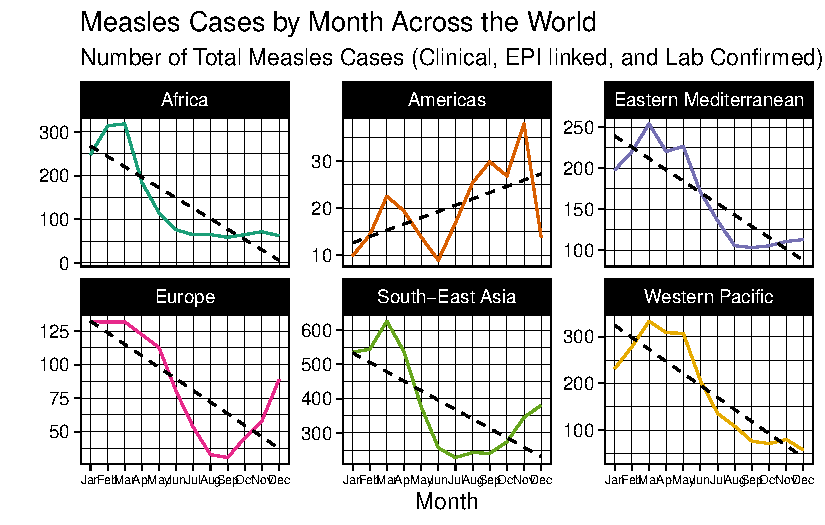
\includegraphics[keepaspectratio,alt={Line plot showing average measles cases by month for each world region (linear model included for each), with separate panels for each region.}]{Measles-Case-Analysis_files/figure-pdf/unnamed-chunk-3-1.pdf}}

}

\caption{Figure 1}

\end{figure}%

Figure 1 shows that all regions except the Americas, there is a negative
trend in measles cases as the months in a year increase, meaning that
the earlier months have seen more measles cases than the later months on
average.

The CDCs resources on Measles may give us some context for our findings,
as the virus is primarily spread through airborne droplets, and is
believed to have originated from the ``Rinderpest'' virus dating back to
before the current era in populated areas of the Eastern hemisphere.

Since we know the Western hemisphere was not the original location of
the virus, the Americas have experienced the lowest amount of measles
cases over time, and country and region-wide data suggest that cases
appear late-in-the-year more often, we are given a solid context for why
this region has experienced the virus differently from the rest of the
world even in the modern age.

\begin{Shaded}
\begin{Highlighting}[]
\NormalTok{largest\_countries }\OtherTok{\textless{}{-}} \FunctionTok{c}\NormalTok{(}\StringTok{"India"}\NormalTok{,}
                       \StringTok{"China"}\NormalTok{,}
                       \StringTok{"United States of America"}\NormalTok{,}
                       \StringTok{"Indonesia"}\NormalTok{,}
                       \StringTok{"Pakistan"}\NormalTok{,}
                       \StringTok{"Nigeria"}\NormalTok{)}

\NormalTok{season\_lookup }\OtherTok{\textless{}{-}} \FunctionTok{tribble}\NormalTok{(}\SpecialCharTok{\textasciitilde{}}\NormalTok{country, }\SpecialCharTok{\textasciitilde{}}\NormalTok{month, }\SpecialCharTok{\textasciitilde{}}\NormalTok{season,}
                         \StringTok{"India"}\NormalTok{, }\StringTok{"Apr"}\NormalTok{, }\StringTok{"Summer"}\NormalTok{,}
                         \StringTok{"India"}\NormalTok{, }\StringTok{"May"}\NormalTok{, }\StringTok{"Summer"}\NormalTok{,}
                         \StringTok{"India"}\NormalTok{, }\StringTok{"Jun"}\NormalTok{, }\StringTok{"Summer"}\NormalTok{,}
                         \StringTok{"India"}\NormalTok{, }\StringTok{"Dec"}\NormalTok{, }\StringTok{"Winter"}\NormalTok{,}
                         \StringTok{"India"}\NormalTok{, }\StringTok{"Jan"}\NormalTok{, }\StringTok{"Winter"}\NormalTok{,}
                         \StringTok{"India"}\NormalTok{, }\StringTok{"Feb"}\NormalTok{, }\StringTok{"Winter"}\NormalTok{,}
                         \StringTok{"China"}\NormalTok{, }\StringTok{"Jun"}\NormalTok{, }\StringTok{"Summer"}\NormalTok{,}
                         \StringTok{"China"}\NormalTok{, }\StringTok{"Jul"}\NormalTok{, }\StringTok{"Summer"}\NormalTok{,}
                         \StringTok{"China"}\NormalTok{, }\StringTok{"Aug"}\NormalTok{, }\StringTok{"Summer"}\NormalTok{,}
                         \StringTok{"China"}\NormalTok{, }\StringTok{"Dec"}\NormalTok{, }\StringTok{"Winter"}\NormalTok{,}
                         \StringTok{"China"}\NormalTok{, }\StringTok{"Jan"}\NormalTok{, }\StringTok{"Winter"}\NormalTok{,}
                         \StringTok{"China"}\NormalTok{, }\StringTok{"Feb"}\NormalTok{, }\StringTok{"Winter"}\NormalTok{,}
                         \StringTok{"United States of America"}\NormalTok{, }\StringTok{"Jun"}\NormalTok{, }\StringTok{"Summer"}\NormalTok{,}
                         \StringTok{"United States of America"}\NormalTok{, }\StringTok{"Jul"}\NormalTok{, }\StringTok{"Summer"}\NormalTok{,}
                         \StringTok{"United States of America"}\NormalTok{, }\StringTok{"Aug"}\NormalTok{, }\StringTok{"Summer"}\NormalTok{,}
                         \StringTok{"United States of America"}\NormalTok{, }\StringTok{"Dec"}\NormalTok{, }\StringTok{"Winter"}\NormalTok{,}
                         \StringTok{"United States of America"}\NormalTok{, }\StringTok{"Jan"}\NormalTok{, }\StringTok{"Winter"}\NormalTok{,}
                         \StringTok{"United States of America"}\NormalTok{, }\StringTok{"Feb"}\NormalTok{, }\StringTok{"Winter"}\NormalTok{,}
                         \StringTok{"Indonesia"}\NormalTok{, }\StringTok{"Sep"}\NormalTok{, }\StringTok{"Summer"}\NormalTok{,}
                         \StringTok{"Indonesia"}\NormalTok{, }\StringTok{"Oct"}\NormalTok{, }\StringTok{"Summer"}\NormalTok{,}
                         \StringTok{"Indonesia"}\NormalTok{, }\StringTok{"Nov"}\NormalTok{, }\StringTok{"Summer"}\NormalTok{,}
                         \StringTok{"Indonesia"}\NormalTok{, }\StringTok{"Jan"}\NormalTok{, }\StringTok{"Winter"}\NormalTok{,}
                         \StringTok{"Indonesia"}\NormalTok{, }\StringTok{"Feb"}\NormalTok{, }\StringTok{"Winter"}\NormalTok{,}
                         \StringTok{"Indonesia"}\NormalTok{, }\StringTok{"Mar"}\NormalTok{, }\StringTok{"Winter"}\NormalTok{,}
                         \StringTok{"Pakistan"}\NormalTok{, }\StringTok{"May"}\NormalTok{, }\StringTok{"Summer"}\NormalTok{,}
                         \StringTok{"Pakistan"}\NormalTok{, }\StringTok{"Jun"}\NormalTok{, }\StringTok{"Summer"}\NormalTok{,}
                         \StringTok{"Pakistan"}\NormalTok{, }\StringTok{"Jul"}\NormalTok{, }\StringTok{"Summer"}\NormalTok{,}
                         \StringTok{"Pakistan"}\NormalTok{, }\StringTok{"Dec"}\NormalTok{, }\StringTok{"Winter"}\NormalTok{,}
                         \StringTok{"Pakistan"}\NormalTok{, }\StringTok{"Jan"}\NormalTok{, }\StringTok{"Winter"}\NormalTok{,}
                         \StringTok{"Pakistan"}\NormalTok{, }\StringTok{"Feb"}\NormalTok{, }\StringTok{"Winter"}\NormalTok{,}
                         \StringTok{"Nigeria"}\NormalTok{, }\StringTok{"Feb"}\NormalTok{, }\StringTok{"Summer"}\NormalTok{,}
                         \StringTok{"Nigeria"}\NormalTok{, }\StringTok{"Mar"}\NormalTok{, }\StringTok{"Summer"}\NormalTok{,}
                         \StringTok{"Nigeria"}\NormalTok{, }\StringTok{"Apr"}\NormalTok{, }\StringTok{"Summer"}\NormalTok{,}
                         \StringTok{"Nigeria"}\NormalTok{, }\StringTok{"Jul"}\NormalTok{, }\StringTok{"Winter"}\NormalTok{,}
                         \StringTok{"Nigeria"}\NormalTok{, }\StringTok{"Aug"}\NormalTok{, }\StringTok{"Winter"}\NormalTok{,}
                         \StringTok{"Nigeria"}\NormalTok{, }\StringTok{"Sep"}\NormalTok{, }\StringTok{"Winter"}\NormalTok{)}

\CommentTok{\#data on seasons from chatgpt: "https://chatgpt.com/share/e/69f554b3{-}799c{-}8002{-}9b3b{-}1c367d53bab9"}
\end{Highlighting}
\end{Shaded}

\begin{Shaded}
\begin{Highlighting}[]
\NormalTok{get\_season }\OtherTok{\textless{}{-}} \ControlFlowTok{function}\NormalTok{(country\_name, month\_name) \{}
  
\NormalTok{  month\_name }\OtherTok{\textless{}{-}} \FunctionTok{as.character}\NormalTok{(month\_name)}
  
\NormalTok{  out }\OtherTok{\textless{}{-}}\NormalTok{ season\_lookup }\SpecialCharTok{|\textgreater{}}
    \FunctionTok{filter}\NormalTok{(country }\SpecialCharTok{==}\NormalTok{ country\_name, month }\SpecialCharTok{==}\NormalTok{ month\_name) }\SpecialCharTok{|\textgreater{}}
    \FunctionTok{pull}\NormalTok{(season)}
  
  \ControlFlowTok{if}\NormalTok{ (}\FunctionTok{length}\NormalTok{(out) }\SpecialCharTok{==} \DecValTok{0}\NormalTok{) \{}
    \FunctionTok{return}\NormalTok{(}\StringTok{"Other"}\NormalTok{)\}}
  \ControlFlowTok{else}\NormalTok{ \{}\FunctionTok{return}\NormalTok{(out[}\DecValTok{1}\NormalTok{])\}}
\NormalTok{  \}}
\end{Highlighting}
\end{Shaded}

\begin{Shaded}
\begin{Highlighting}[]
\NormalTok{country\_month\_summary }\OtherTok{\textless{}{-}}\NormalTok{ cases\_month }\SpecialCharTok{|\textgreater{}}
  \FunctionTok{filter}\NormalTok{(country }\SpecialCharTok{\%in\%}\NormalTok{ largest\_countries) }\SpecialCharTok{|\textgreater{}}
  \FunctionTok{group\_by}\NormalTok{(month, country) }\SpecialCharTok{|\textgreater{}}
  \FunctionTok{summarise}\NormalTok{(}\AttributeTok{avg\_measles =} \FunctionTok{mean}\NormalTok{(measles\_total, }\AttributeTok{na.rm =} \ConstantTok{TRUE}\NormalTok{), }\AttributeTok{.groups =} \StringTok{"drop"}\NormalTok{) }\SpecialCharTok{|\textgreater{}}
  \FunctionTok{mutate}\NormalTok{(}\AttributeTok{month =} \FunctionTok{factor}\NormalTok{(month.abb[month], }\AttributeTok{levels =}\NormalTok{ month.abb))}

\NormalTok{country\_month\_summary }\OtherTok{\textless{}{-}}\NormalTok{ country\_month\_summary }\SpecialCharTok{|\textgreater{}}
  \FunctionTok{mutate}\NormalTok{(}\AttributeTok{season =} \FunctionTok{map2\_chr}\NormalTok{(country, }\FunctionTok{as.character}\NormalTok{(month), get\_season))}

\NormalTok{country\_month\_summary }\SpecialCharTok{|\textgreater{}}
  \FunctionTok{group\_by}\NormalTok{(season) }\SpecialCharTok{|\textgreater{}}
  \FunctionTok{summarize}\NormalTok{(}\AttributeTok{avg\_measles =} \FunctionTok{mean}\NormalTok{(avg\_measles)) }\SpecialCharTok{|\textgreater{}}
  \FunctionTok{gt}\NormalTok{() }\SpecialCharTok{|\textgreater{}}
  \FunctionTok{fmt\_number}\NormalTok{(}\AttributeTok{columns =}\NormalTok{ avg\_measles, }\AttributeTok{decimals =} \DecValTok{2}\NormalTok{) }\SpecialCharTok{|\textgreater{}}
  \FunctionTok{cols\_label}\NormalTok{(}\AttributeTok{season =} \StringTok{"Season"}\NormalTok{,}
             \AttributeTok{avg\_measles =} \StringTok{"Average Measles Cases"}\NormalTok{) }\SpecialCharTok{|\textgreater{}}
  \FunctionTok{tab\_header}\NormalTok{(}\AttributeTok{title =} \StringTok{"Average Monthly Measles Cases per Country by Season"}\NormalTok{,}
             \AttributeTok{subtitle =} \StringTok{"Based on the six most populous countries in the dataset"}\NormalTok{) }\SpecialCharTok{|\textgreater{}}
  \FunctionTok{tab\_style}\NormalTok{(}\AttributeTok{style =} \FunctionTok{cell\_text}\NormalTok{(}\AttributeTok{weight =} \StringTok{"bold"}\NormalTok{),}
            \AttributeTok{locations =} \FunctionTok{cells\_title}\NormalTok{(}\AttributeTok{groups =} \StringTok{"title"}\NormalTok{))}
\end{Highlighting}
\end{Shaded}

\begin{table}
\caption*{
{\fontsize{20}{25}\selectfont  Average Monthly Measles Cases per Country by Season\fontsize{12}{15}\selectfont } \\ 
{\fontsize{14}{17}\selectfont  Based on the six most populous countries in the dataset\fontsize{12}{15}\selectfont }
} 
\fontsize{12.0pt}{14.0pt}\selectfont
\begin{tabular*}{\linewidth}{@{\extracolsep{\fill}}lr}
\toprule
Season & Average Measles Cases \\ 
\midrule\addlinespace[2.5pt]
Other & 1,022.95 \\ 
Summer & 1,468.26 \\ 
Winter & 1,231.95 \\ 
\bottomrule
\end{tabular*}
\end{table}

Table 2

\begin{Shaded}
\begin{Highlighting}[]
\NormalTok{country\_month\_summary }\SpecialCharTok{|\textgreater{}}
  \FunctionTok{ggplot}\NormalTok{(}\FunctionTok{aes}\NormalTok{(}\AttributeTok{x =}\NormalTok{ season, }\AttributeTok{y =}\NormalTok{ avg\_measles, }\AttributeTok{fill =}\NormalTok{ season)) }\SpecialCharTok{+}
  \FunctionTok{geom\_violin}\NormalTok{(}\AttributeTok{trim =} \ConstantTok{FALSE}\NormalTok{, }\AttributeTok{alpha =} \FloatTok{0.7}\NormalTok{) }\SpecialCharTok{+}
  \FunctionTok{labs}\NormalTok{(}\AttributeTok{title =} \StringTok{"Average Measles Cases per Country by Season"}\NormalTok{,}
       \AttributeTok{subtitle =} \StringTok{"Summer and winter determined by average temperature, data from six representative countries"}\NormalTok{,}
       \AttributeTok{x =} \StringTok{"Season"}\NormalTok{,}
       \AttributeTok{y =} \StringTok{""}\NormalTok{) }\SpecialCharTok{+}
  \FunctionTok{scale\_fill\_brewer}\NormalTok{(}\AttributeTok{palette =} \StringTok{"Dark2"}\NormalTok{) }\SpecialCharTok{+}
  \FunctionTok{theme\_bw}\NormalTok{() }\SpecialCharTok{+}
  \FunctionTok{theme}\NormalTok{(}\AttributeTok{legend.position =} \StringTok{"none"}\NormalTok{)}
\end{Highlighting}
\end{Shaded}

\begin{figure}[H]

{\centering \pandocbounded{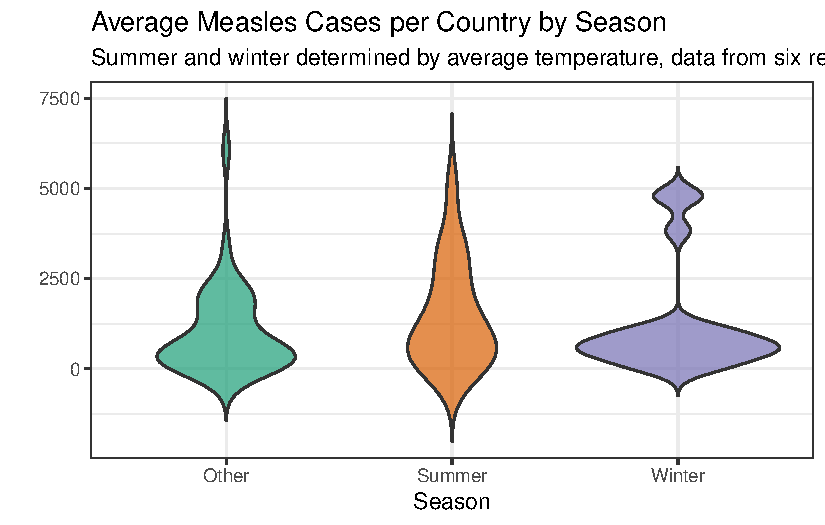
\includegraphics[keepaspectratio,alt={Violin plot showing distrobution of measles cases bases on season for six representative countries}]{Measles-Case-Analysis_files/figure-pdf/unnamed-chunk-7-1.pdf}}

}

\caption{Figure 2}

\end{figure}%

We can see in figure 2 that the distributions of measles cases bases on
season have slightly different shapes, but are overall quite similar.
Non-winter months tend to be pretty varied in their measles
distribution, while winter months have typical values, followed by a
gap, and then spiked values. This may indicate that winter often sees
typical measles counts but has seen a few outbreaks over the years as
well.

\subsubsection{Statistical Significance of Month and
Season}\label{statistical-significance-of-month-and-season}

\begin{Shaded}
\begin{Highlighting}[]
\CommentTok{\#summary(aov(measles\_total \textasciitilde{} month, data = cases\_month))}
\CommentTok{\#summary(aov(avg\_measles \textasciitilde{} season, data = country\_month\_summary))}

\NormalTok{anova\_results }\OtherTok{\textless{}{-}} \FunctionTok{tibble}\NormalTok{(}
  \AttributeTok{Model =} \FunctionTok{c}\NormalTok{(}\StringTok{"Month"}\NormalTok{, }\StringTok{"Season"}\NormalTok{),}
  \AttributeTok{Predictor =} \FunctionTok{c}\NormalTok{(}\StringTok{"Month"}\NormalTok{, }\StringTok{"Season"}\NormalTok{),}
  \AttributeTok{DF\_numerator =} \FunctionTok{c}\NormalTok{(}\DecValTok{1}\NormalTok{, }\DecValTok{2}\NormalTok{),}
  \AttributeTok{DF\_denominator =} \FunctionTok{c}\NormalTok{(}\DecValTok{22630}\NormalTok{, }\DecValTok{69}\NormalTok{),}
  \AttributeTok{F\_statistic =} \FunctionTok{c}\NormalTok{(}\FloatTok{68.34}\NormalTok{, }\FloatTok{0.658}\NormalTok{),}
  \AttributeTok{p\_value =} \FunctionTok{c}\NormalTok{(}\StringTok{"\textless{} 2e{-}16"}\NormalTok{, }\StringTok{"0.521"}\NormalTok{),}
  \AttributeTok{Conclusion =} \FunctionTok{c}\NormalTok{(}\StringTok{"Significant"}\NormalTok{, }\StringTok{"Not significant"}\NormalTok{))}

\NormalTok{anova\_results }\SpecialCharTok{|\textgreater{}}
  \FunctionTok{gt}\NormalTok{() }\SpecialCharTok{|\textgreater{}}
  \FunctionTok{cols\_label}\NormalTok{(}\AttributeTok{DF\_numerator =} \StringTok{"DF numerator"}\NormalTok{,}
             \AttributeTok{DF\_denominator =} \StringTok{"DF denominator"}\NormalTok{,}
             \AttributeTok{F\_statistic =} \StringTok{"F statistic"}\NormalTok{,}
             \AttributeTok{p\_value =} \StringTok{"p{-}value"}\NormalTok{) }\SpecialCharTok{|\textgreater{}}
  \FunctionTok{tab\_header}\NormalTok{(}\AttributeTok{title =} \StringTok{"Testing for Significance"}\NormalTok{) }\SpecialCharTok{|\textgreater{}}
  \FunctionTok{tab\_style}\NormalTok{(}\AttributeTok{style =} \FunctionTok{cell\_text}\NormalTok{(}\AttributeTok{weight =} \StringTok{"bold"}\NormalTok{),}
            \AttributeTok{locations =} \FunctionTok{cells\_title}\NormalTok{(}\AttributeTok{groups =} \StringTok{"title"}\NormalTok{))}
\end{Highlighting}
\end{Shaded}

\begin{table}
\caption*{
{\fontsize{20}{25}\selectfont  Testing for Significance\fontsize{12}{15}\selectfont }
} 
\fontsize{12.0pt}{14.0pt}\selectfont
\begin{tabular*}{\linewidth}{@{\extracolsep{\fill}}llrrrll}
\toprule
Model & Predictor & DF numerator & DF denominator & F statistic & p-value & Conclusion \\ 
\midrule\addlinespace[2.5pt]
Month & Month & 1 & 22630 & 68.340 & < 2e-16 & Significant \\ 
Season & Season & 2 & 69 & 0.658 & 0.521 & Not significant \\ 
\bottomrule
\end{tabular*}
\end{table}

Table 3

The F tests indicate that month is a significant predictor of measles
cases in the overall monthly model, while the season variable was not
significant in the six country model. This means the data provide strong
evidence that measles cases vary across the year, but this simplified
winter/summer/other classification does not explain enough variation to
be statistically significant. Because the season model was based on only
six countries and a rough season grouping, this result may be worth
investigating further. Overall, the results suggest that calendar month
may capture the timing of measles incidence better than this
country-specific season variable. This makes sense because measles is a
highly contagious virus, so a spike in one country is likely to spread
to many others in the same month, regardless of the current season in
the country to which it spreads.




\end{document}
